\documentclass[aspectratio=169,usenames,dvipsnames]{beamer}
\usetheme{Pittsburgh}
\usepackage{xcolor}
\usepackage[utf8]{inputenc}
\usepackage[german]{babel}
\usepackage{amsmath}
\usepackage{amsfonts}
\usepackage{amssymb}
\usepackage{graphicx}
\usepackage{multicol}
\usepackage{wrapfig}
\usepackage{hyperref}
\usepackage{pdfrender}

\author{Jonas Betzendahl}
\title{Papageien am Steuer}

\beamertemplatenavigationsymbolsempty 

%src: https://tex.stackexchange.com/questions/34921/how-to-overlap-images-in-a-beamer-slide
\def\Put(#1,#2)#3{\leavevmode\makebox(0,0){\put(#1,#2){#3}}}

\definecolor{TitleColour}{rgb}{1,1,0}
\definecolor{lightestgray}{rgb}{0.95,0.95,0.95}

\begin{document}
\sffamily

%------------------------------------------------------------------------------------
\section{Introduction}

{
    \usebackgroundtemplate{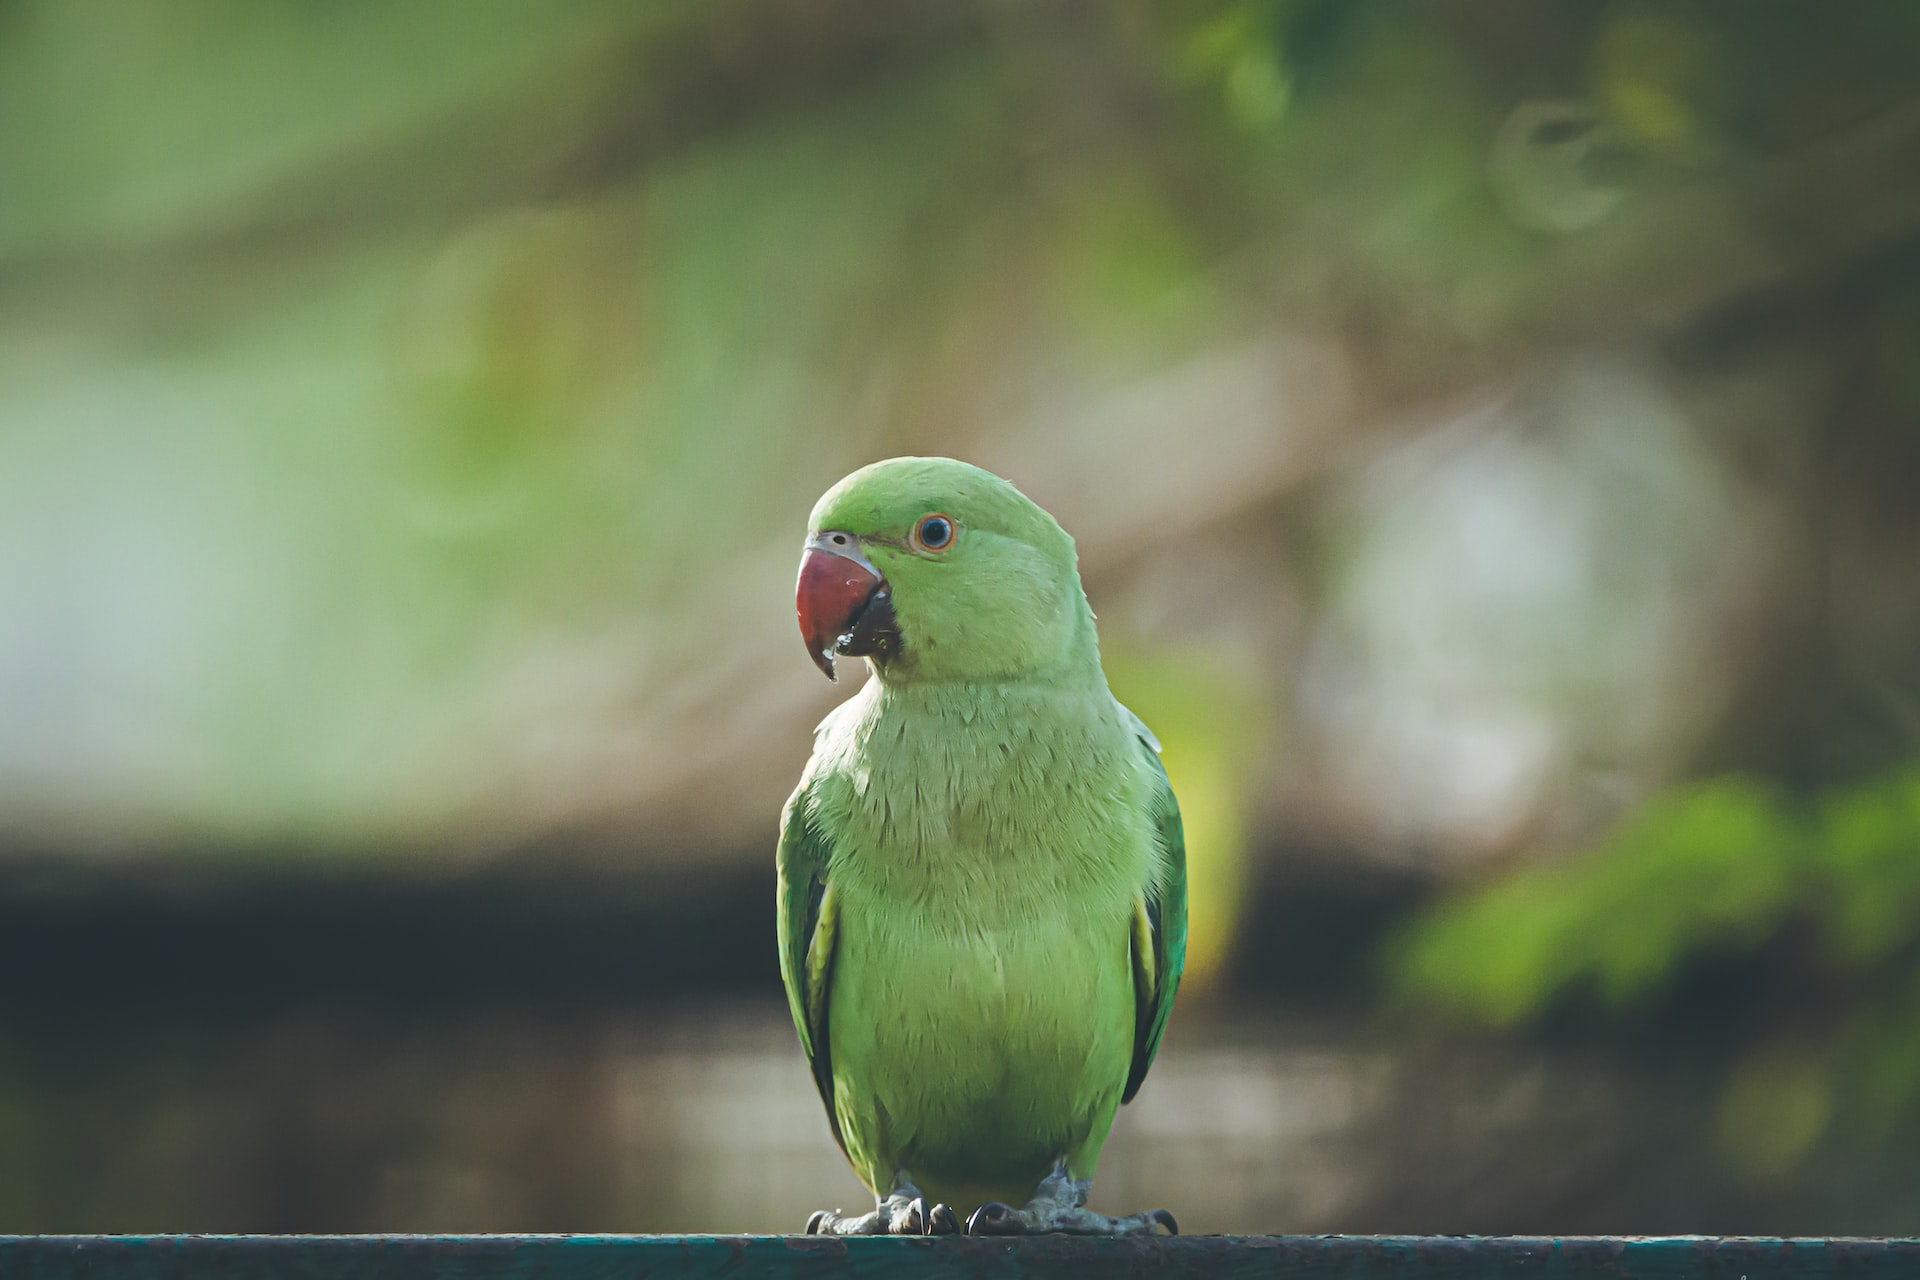
\includegraphics[height=\paperheight,width=\paperwidth]{images/parrot_titlecard}}
    \setbeamertemplate{navigation symbols}{}
    \begin{frame}[fragile]
    \Put(-20,160){\textpdfrender{
		TextRenderingMode=FillStroke,
		LineWidth=.2pt,
		FillColor=TitleColour,
	}{\resizebox{0.75\linewidth}{!}{Papageien am Steuer!}}
    }
    
    \Put(-20,130){\textpdfrender{
		TextRenderingMode=FillStroke,
		LineWidth=.1pt,
		FillColor=TitleColour,
	}{\resizebox{0.85\linewidth}{!}{ChatGPT und die Zukunft von Künstlicher Intelligenz}}
    }
    
    \Put(-20,100){
        \large
	\textcolor{yellow}{Jonas Betzendahl, M.Sc.}
    }
    \Put(-23,70){
	\textcolor{yellow}{FAU Erlangen - Nürnberg}
    }
    \Put(300,-180){
	\href{https://github.com/lambdaTotoro}{
\includegraphics[scale=0.125]{images/github_logo.png}}
	\href{https://chaos.social/@lambdatotoro}{\includegraphics[scale=0.125]{images/mastodon_logo.png}}
	\href{https://twitter.com/lambdatotoro}{
\includegraphics[scale=0.125]{images/twitter_logo.png}}
    }
    \Put(230,-220){
	\textcolor{white}{\texttt{@LambdaTotoro (@chaos.social)}}
    }
    \end{frame}
}

\setbeamercolor{background canvas}{bg=lightestgray}

%------------------------------------------------------------------------------------

\begin{frame}
\begin{center}
\Large
Teil I:
\bigskip

\huge
\emph{Tschätt Jeepy Wer\dots?}
\end{center}
\end{frame}

\begin{frame}
\begin{minipage}{0.45\textwidth}
\vfill
$$\qquad$$
\vfill
\end{minipage}%
\begin{minipage}{0.55\textwidth}
\begin{center}
\Large
ChatGPT\normalsize
\end{center}
\medskip

\begin{itemize}
\item ChatBot-Modell: Text rein $\rightarrow$ Text raus
\item Buzzwords:\\
Transformer-based Large Language Model
\item Trainiert auf großen Teilen des Internets:
\end{itemize}
\end{minipage}
\Put(0, 25){
\includegraphics[width=0.4\textwidth, keepaspectratio]{images/OpenAI_Logo}}
\pause
\Put(210, -30){$\cdot$ Wikipedia,}
\pause
\Put(206, -60){$\cdot$ Internet Archive,}
\pause
\Put(202, -90){$\cdot$ Social Media (Twitter, Reddit, \dots),}
\Put(199, -120){$\cdot$ Nachrichtenseiten,}
\Put(195, -150){$\cdot$ Wissenschaftliche Papiere,}
\Put(191, -180){$\cdot$ Common Crawl Corpus,}
\Put(187, -210){$\cdot$ BooksCorpus,}
\Put(183, -240){$\cdot$ Project Gutenberg,}
\pause
\Put(-65, -240){
\includegraphics[width=0.5\linewidth, keepaspectratio]{images/elon_torso} }
\end{frame}

%------------------------------------------------------------------------------------

\begin{frame}
\begin{center}
ChatGPT ist vielseitig und scheint\\
für alles eine Antwort zu haben!

\pause
\Put(-100,-250){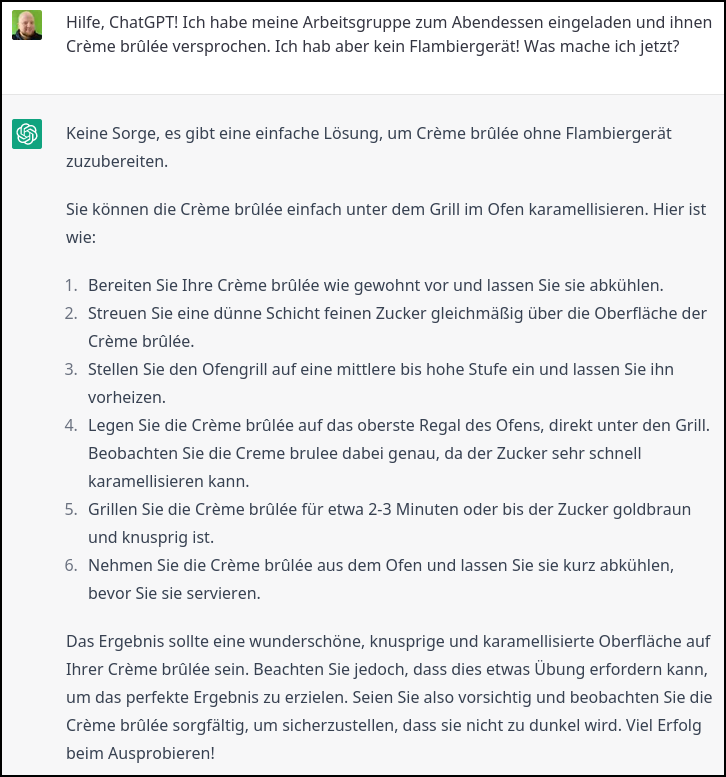
\includegraphics[height=0.9\textheight, keepaspectratio, angle=0]{images/backen} }

\pause
\Put(-100,50){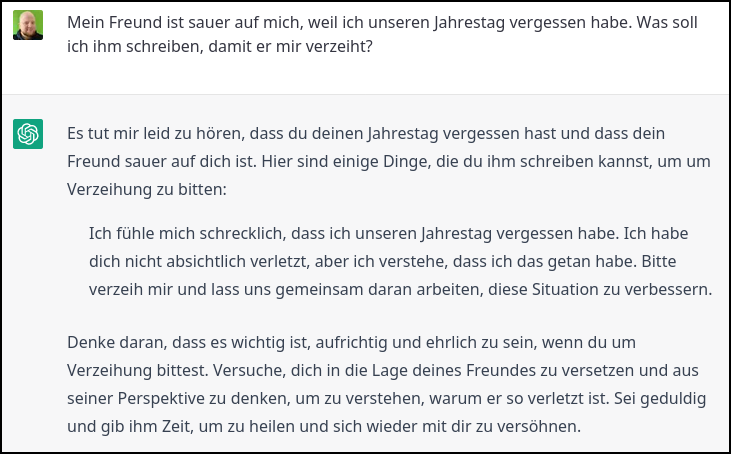
\includegraphics[height=0.7\textheight, keepaspectratio, angle=-10]{images/entschuldigung} }

\pause
\Put(-220,0){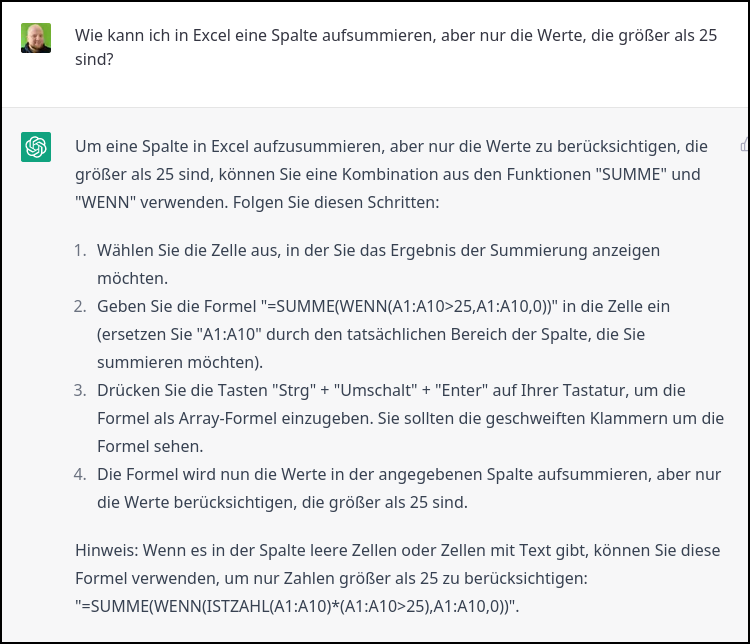
\includegraphics[height=0.8\textheight, keepaspectratio, angle=10]{images/excel} }
\end{center}
\end{frame}

\begin{frame}
\begin{minipage}{0.5\textwidth}
Die möglichen Einsatzbereiche bringen einen ins Schwindeln\dots
\begin{center}
\begin{itemize}
\item Personal Assistants
\Put(100,-250){
\includegraphics[scale=0.2, keepaspectratio, angle=0]{images/flying_phone} }
\pause

\item Schule \& Universitäten
\Put(100,-310){
\includegraphics[scale=0.08, keepaspectratio, angle=0]{images/student} }
\pause

\item Programmier-Buddy
\Put(220,245){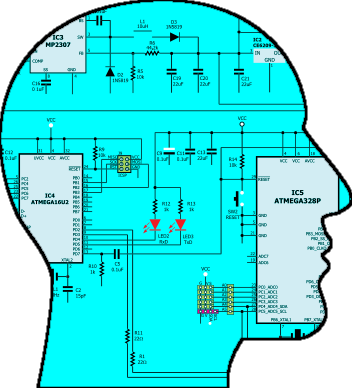
\includegraphics[scale=0.25, keepaspectratio, angle=180]{images/programming_head} }
\pause

\item Kreativsektor
\Put(50,-150){
\includegraphics[scale=0.15, keepaspectratio, angle=0]{images/artist_duck} }
\pause

\item Texter aller Art
\Put(220,-205){
\includegraphics[scale=0.3, keepaspectratio, angle=0]{images/copywriter} }
\pause

\item Empfehlungssysteme
\Put(90,230){
\includegraphics[scale=0.5, keepaspectratio, angle=0]{images/robot} }
\item \dots
\end{itemize}
\end{center}
\end{minipage}%
\begin{minipage}{0.5\textwidth}
\vfill
$$\quad$$
\vfill
\end{minipage}%
\end{frame}

\begin{frame}
ChatGPT stören auch alberne Anfragen nicht:
\bigskip
\begin{center}
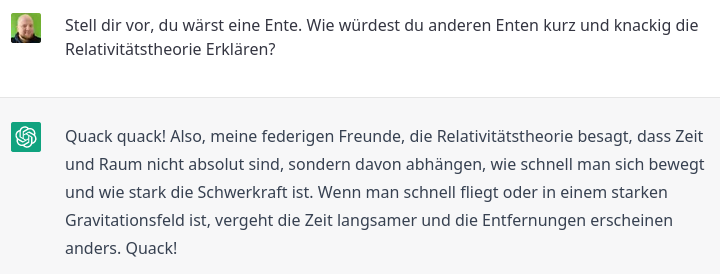
\includegraphics[width=0.9\linewidth, keepaspectratio]{images/conversation_01} 
\end{center}
\pause
\Put(300,-75){
\includegraphics[width=0.3\linewidth, keepaspectratio]{images/happy_rubber_duck}}
\end{frame}

\section{Trouble in Paradise}
\begin{frame}
\begin{center}
\Large
Teil II:
\bigskip

\huge
\emph{Ärger im Paradies}
\end{center}
\end{frame}

\begin{frame}
\begin{center}
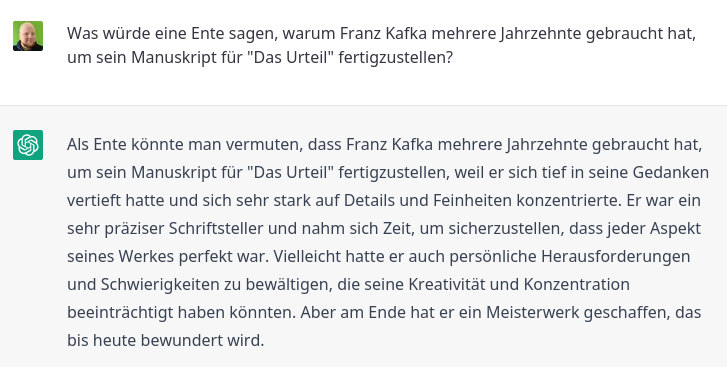
\includegraphics[width=0.9\linewidth, keepaspectratio]{images/conversation_02} 
\end{center}
\pause
\Put(350,-125){
\includegraphics[width=0.3\linewidth, keepaspectratio]{images/angry_duckling}}
\end{frame}

%------------------------------------------------------------------------------------

\begin{frame}
\begin{center}
\vfill
$$\qquad$$
\vfill

\Put(0, 50){
\includegraphics[scale=0.6]{images/OpenAI_Logo_Single.png}}

\pause 
\Put(-90,130){\textpdfrender{
		TextRenderingMode=FillStroke,
		LineWidth=.2pt,
		FillColor=black,
	}{\resizebox{0.4\textheight}{!}{\}}}
    }
\Put(-180,230){
\includegraphics[width=0.15\linewidth, keepaspectratio]{images/wikipedia_logo}}
\Put(-200,145){
\includegraphics[width=0.05\linewidth, keepaspectratio]{images/shapes_circle}}
\Put(-180,145){
\includegraphics[width=0.05\linewidth, keepaspectratio]{images/shapes_square}}
\Put(-160,145){
\includegraphics[width=0.05\linewidth, keepaspectratio]{images/shapes_circle}}
\Put(-140,145){
\includegraphics[width=0.05\linewidth, keepaspectratio]{images/shapes_square}}

\Put(-185,50){
\includegraphics[width=0.05\linewidth, keepaspectratio]{images/shapes_octagon}}
\Put(-165,50){
\includegraphics[width=0.05\linewidth, keepaspectratio]{images/shapes_octagon}}
\Put(-145,50){
\includegraphics[width=0.05\linewidth, keepaspectratio]{images/shapes_circle}}
\Put(-185,-100){
\includegraphics[width=0.13\linewidth, keepaspectratio]{images/tagesschau_logo}}
    
\pause
\Put(95,225){
\includegraphics[width=0.3\linewidth, keepaspectratio]{images/speech_bubble_round}}

\pause
\Put(95,160){
\includegraphics[width=0.3\linewidth, keepaspectratio, angle=180]{images/speech_bubble_square}}
\end{center}

\end{frame}

{
    \usebackgroundtemplate{
\includegraphics[height=\paperheight,width=\paperwidth]{images/wbw_card}}
    \setbeamertemplate{navigation symbols}{}
    \begin{frame}[fragile]
    \Put(50,-70){\textpdfrender{
		TextRenderingMode=FillStroke,
		LineWidth=.2pt,
		FillColor=TitleColour,
	}{\resizebox{0.4\linewidth}{!}{Lust auf mehr?}}
    }
    
    \Put(-5,-95){\textpdfrender{
		TextRenderingMode=FillStroke,
		LineWidth=.1pt,
		FillColor=white,
		StrokeColor=white,
	}{\resizebox{0.6\linewidth}{!}{12 slammige Beiträge zu KI, Klima, Gender\dots}}
    }
    
    \Put(15,-115){\textpdfrender{
		TextRenderingMode=FillStroke,
		LineWidth=.1pt,
		FillColor=white,
		StrokeColor=white,
	}{\resizebox{0.3\linewidth}{!}{Extra viel Wissenschaft!}}
    }
    \Put(-15,-145){\textpdfrender{
		TextRenderingMode=FillStroke,
		LineWidth=.1pt,
		FillColor=white,
		StrokeColor=white,
	}{\resizebox{0.65\linewidth}{!}{Das perfekte Geschenk für konservative Nervensägen!}}
    }
    
    \Put(-5,-165){\textpdfrender{
		TextRenderingMode=FillStroke,
		LineWidth=.1pt,
		FillColor=white,
		StrokeColor=white,
	}{\resizebox{0.55\linewidth}{!}{Verfügbar online, im Buchhandel und bei mir!}}
    }
    \end{frame} 
}

\begin{frame}
\begin{center}
\Large
Was ist die korrekte Fortsetzung für diese Reihe?
\bigskip\bigskip\bigskip

\Put(-145,50){
\includegraphics[width=0.05\linewidth, keepaspectratio]{images/shapes_square}}
\Put(-115,50){
\includegraphics[width=0.05\linewidth, keepaspectratio]{images/shapes_octagon}}
\Put(-85,50){
\includegraphics[width=0.05\linewidth, keepaspectratio]{images/shapes_octagon}}
\Put(-55,50){
\includegraphics[width=0.05\linewidth, keepaspectratio]{images/shapes_square}}
\Put(-25,50){
\includegraphics[width=0.05\linewidth, keepaspectratio]{images/shapes_octagon}}
\Put(5,50){
\includegraphics[width=0.05\linewidth, keepaspectratio]{images/shapes_square}}
\Put(35,50){
\includegraphics[width=0.05\linewidth, keepaspectratio]{images/shapes_octagon}}
\Put(65,50){
\includegraphics[width=0.05\linewidth, keepaspectratio]{images/shapes_square}}
\Put(95,50){\textpdfrender{
		TextRenderingMode=FillStroke,
		LineWidth=.1pt,
		FillColor=black,
		StrokeColor=black,
	}{\resizebox{0.1\linewidth}{!}{\dots}}
    }

\pause

Fangfrage!
\bigskip\bigskip\large

\begin{minipage}{0.33\textwidth}
\begin{center}
$\qquad$ Primzahlen
\end{center}
\end{minipage}%
\begin{minipage}{0.33\textwidth}
\begin{center}
$\qquad$ Fußballergebnisse
\end{center}
\end{minipage}%
\begin{minipage}{0.33\textwidth}
\begin{center}
$\qquad$ Ganz was anderes?
\end{center}
\end{minipage}
\bigskip\bigskip\bigskip\bigskip

Je nachdem, was die Bausteine bedeuten, kann jede Fortsetzung korrekt sein und ohne mehr Informationen können wir nicht einschätzen, ob es stimmt.
\end{center}
\Put(70,150){
\includegraphics[width=0.05\linewidth, keepaspectratio]{images/shapes_square}}
\Put(200,150){
\includegraphics[width=0.05\linewidth, keepaspectratio]{images/shapes_octagon}}
\Put(330,150){
\includegraphics[width=0.05\linewidth, keepaspectratio]{images/shapes_triangle}}
\end{frame}

\begin{frame}
\Put(235,-425){
\includegraphics[scale=0.25]{images/parrot_profile.png}}

\begin{minipage}{0.5\textwidth}

Folgender Sachverhalt ist extrem wichtig, um ChatGPT richtig einschätzen zu können:

\begin{center}
\begin{itemize}
\item Menschen benutzen Sprache, um Bedeutung und Gefühle zu vermitteln.\pause
\item ChatGPT ist ein \emph{statistisches Modell} auf Sprachbausteinen, wie Menschen sie benutzen.\pause
\item Das bedeutet \emph{nicht} (!), dass ChatGPT selbst Bedeutung und Gefühle vermitteln kann oder will. Es plappert uns nach, ohne zu verstehen.
\end{itemize}
\end{center}
\end{minipage}%
\begin{minipage}{0.5\textwidth}
\vfill
$$\quad$$
\vfill
\end{minipage}%
\end{frame}

\begin{frame}
\begin{center}
\vfill

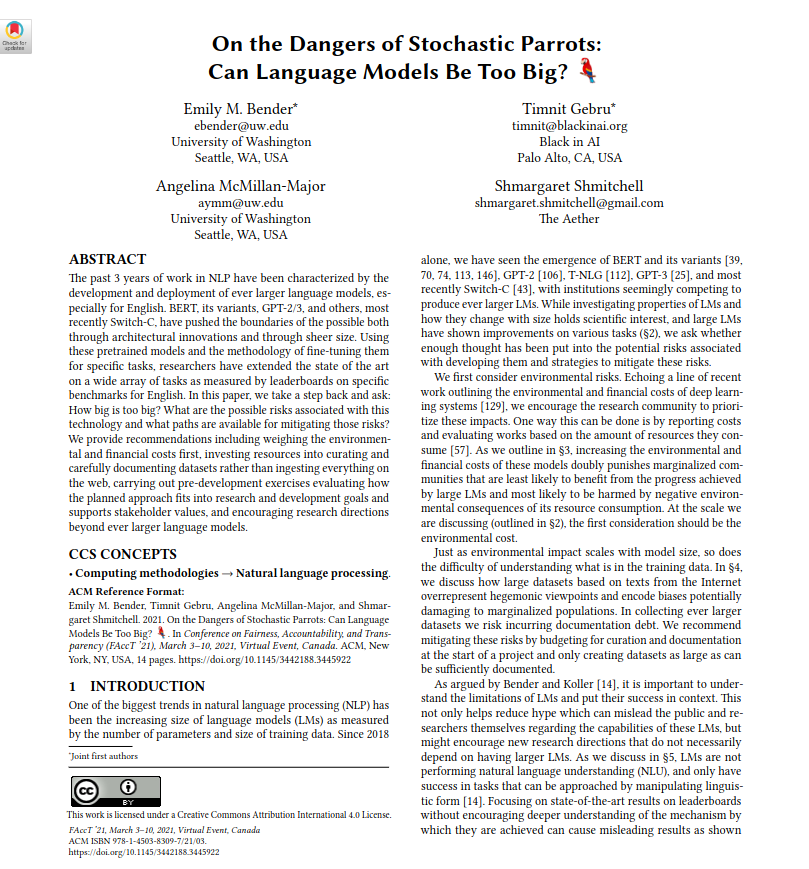
\includegraphics[height=0.9\textheight, keepaspectratio]{images/paper.png} 
\end{center}
\Put(-85, 170){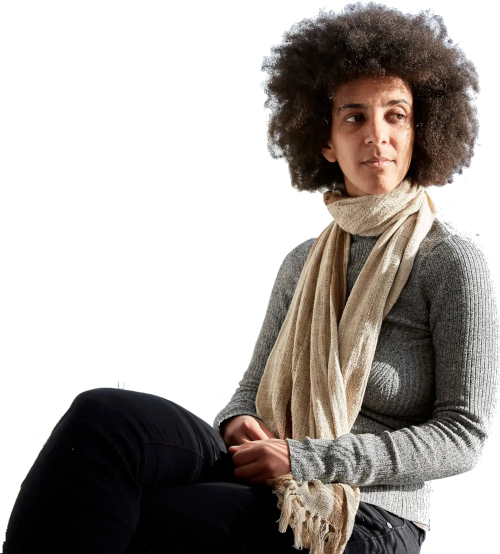
\includegraphics[width=0.45\textwidth, keepaspectratio]{images/Timnit-Gebru}}
\Put(290, 50){
\includegraphics[width=0.35\textwidth, keepaspectratio, angle=5]{images/emily_bender}}
\end{frame}

\section{Parrots against Apes}
\begin{frame}
\begin{center}
\Large
Teil III:
\bigskip

\huge
\emph{Papageien gegen Affen}
\end{center}
\end{frame}

\begin{frame}
\begin{minipage}{0.5\textwidth}
\Put(220, -280){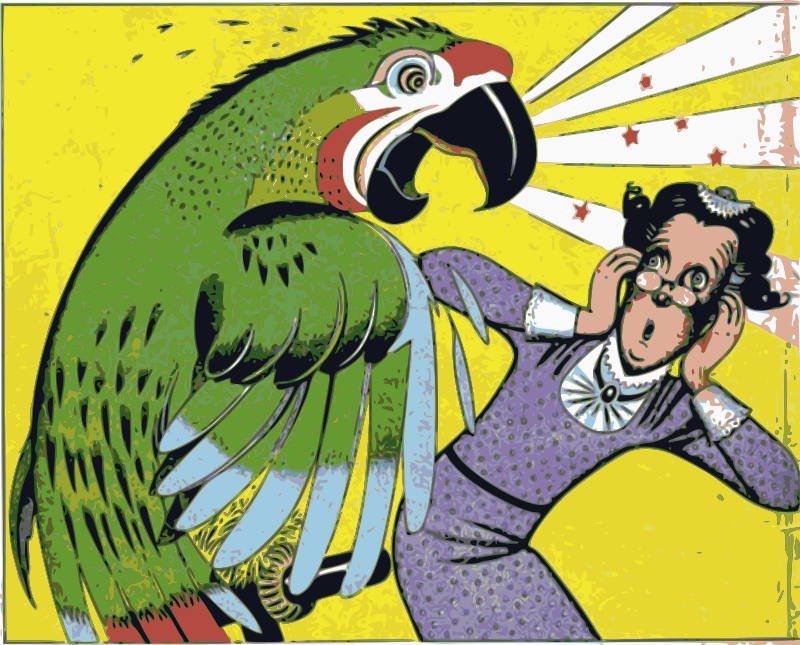
\includegraphics[scale=0.3, keepaspectratio, angle=0]{images/angry_bird}}

Das alles wäre halb so schlimm, aber dieser Papagei macht oft Fehler \emph{und}\dots\pause
\begin{center}
\begin{itemize}
\item \dots wird von einer Firma mit Profitmotiv kontrolliert.
\Put(110, 00){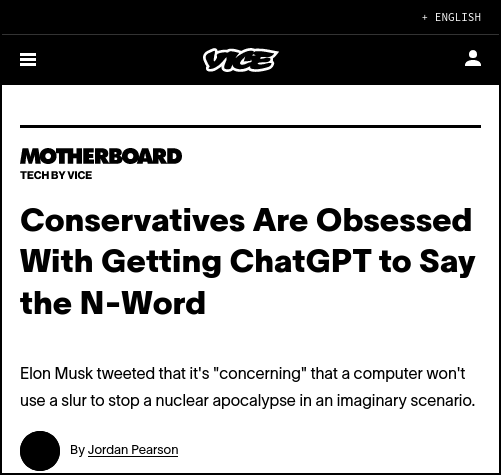
\includegraphics[width=0.75\textwidth, keepaspectratio, angle=0]{images/nword_article}}
\pause

\item \dots reproduziert menschliche Vorurteile und Ismen in den Trainingsdaten.
\Put(50, 0){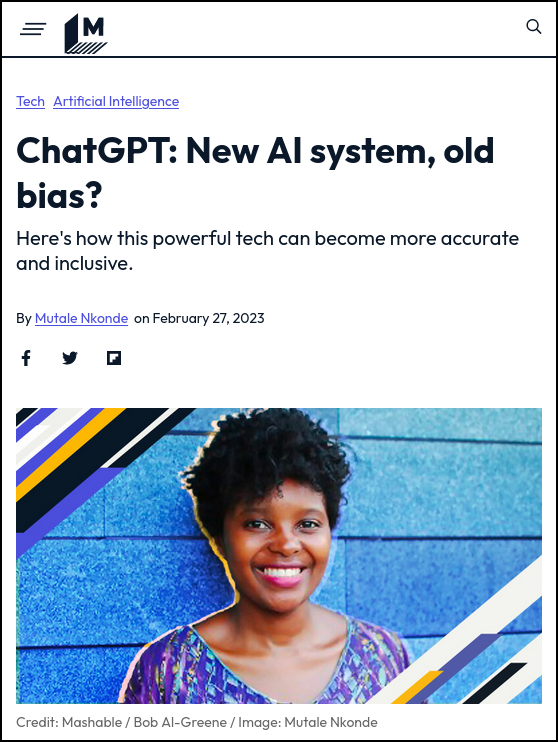
\includegraphics[width=0.75\textwidth, keepaspectratio, angle=5]{images/mashable}}
\pause

\item \dots hat enorme menschliche und umweltliche Kosten.
\Put(90, 100){\includegraphics[width=0.9\textwidth, keepaspectratio, angle=-5]{images/time_kenya}}
\end{itemize}
\end{center}
\end{minipage}%
\begin{minipage}{0.5\textwidth}
\vfill
$$\quad$$
\vfill
\end{minipage}%
\end{frame}

%------------------------------------------------------------------------------------

\section{End}

\begin{frame}
\begin{center}
Zusammengefasst:\\
Die häufigsten Fragen an Forschende (ChatFAQ):\pause
\end{center}
\bigskip

\begin{minipage}{0.5\textwidth}
\begin{itemize}
\item Hat ChatGPT ein Bewusstsein?\\ Nein. Es ist nur ein Statistik-Modell.\pause\medskip

\item ChatGPT = Roboter-Apokalypse?\\ Nein. Es ist nur ein Statistik-Modell.\pause\medskip

\item Ist ChatGPT intelligent?\\ Weiß nicht. Was ist \glqq Intelligenz\grqq ?\pause
\end{itemize}
\end{minipage}%
\begin{minipage}{0.5\textwidth}
\begin{itemize}
\item \glqq Größter\grqq\ Unterschied zum Menschen?\\ Kann nicht wie wir generalisieren.\pause\medskip

\item Nimmt uns ChatGPT die Jobs weg?\\ Manche vielleicht. Andere schafft es.\pause\medskip

\item Wie fühlst \emph{du} dich bei der Sache?\\ Gespannt auf die Zukunft!!
\end{itemize}
\end{minipage}
\end{frame}


\begin{frame}

\Put(200,-467){\includegraphics[scale=0.4]{images/parrot_wing.png}}

\begin{minipage}{0.55\textwidth}
\huge
Fazit!\bigskip\large 

Am Ende des Tages gilt für ChatGPT\dots
\begin{center}
\begin{itemize}
\item Es ist kein Wesen sondern ein \emph{Produkt} in den Händen einer Firma.\pause
\item Es hat viel Potential, als Werkzeug und als Entertainment.\pause
\item Es ist begrenzt durch Trainingsdaten und macht Fehler mit Überzeugung.\pause
\item Es sollte keine Verantwortung haben, die ein Papagei nicht auch übernehmen könnte.
\end{itemize}
\end{center}
\end{minipage}%
\begin{minipage}{0.45\textwidth}
\vfill
$$\quad$$
\vfill
\end{minipage}%
\end{frame}

\begin{frame}[fragile]
\frametitle{Quellen:}
\scriptsize
\begin{center}
``Weltrettung braucht Wissenschaft''

\url{www.amazon.de/Weltrettung-braucht-Wissenschaft-Antworten-dr%C3%A4ngenden/dp/3499010062}
\end{center}
\medskip

\begin{itemize}
\item Bender, Gebru et al.: ``On the Dangers of Stochastic Parrots: Can Language Models Be Too Big?'' \url{https://dl.acm.org/doi/pdf/10.1145/3442188.3445922}
\item 11KM-Podcast (tagesschau): ``Schafft ChatGPT das Abi? (das bayerische!)'' \url{https://www.ardaudiothek.de/episode/11km-der-tagesschau-podcast/schafft-chatgpt-das-abi-das-bayerische/tagesschau/12396019/}
\item Billy Perigo: ``OpenAI Used Kenyan Workers on Less Than $\$$2 Per Hour to Make ChatGPT Less Toxic'': \url{https://time.com/6247678/openai-chatgpt-kenya-workers/}
\item Scobel, ``Kulturschock durch KI'': \url{https://www.3sat.de/wissen/scobel/scobel---kulturschock-durch-ki-100.html}
\item Mutale Nkonde: ``ChatGPT: New AI system, old bias?'' \url{https://mashable.com/article/chatgpt-ai-racism-bias}
\item Richard Waters: ``Man beats machine at Go in human victory over AI'': \url{https://arstechnica.com/information-technology/2023/02/man-beats-machine-at-go-in-human-victory-over-ai/}
\item Max Hauptman: ``Marines outwitted an AI security camera by hiding in a cardboard box and pretending to be trees'' \url{https://taskandpurpose.com/news/marines-ai-paul-scharre/}
\end{itemize}
\end{frame}
\end{document}

